%%% ----------
\section{ПРОГРАММА <<АВАНТ-КОНФИГУРАТОР>>}	\label{sec:configurator}

Просмотр содержимого журналов данных, просмотр текущего состояния, просмотр и изменение параметров, изменение режима работы приемопередатчика осуществляется с помощью персонального компьютера (ПК) с установленной специализированной программой <<АВАНТ-конфигуратор>> (далее конфигуратор).

Конфигуратор состоит из нескольких страниц, между которыми можно свободно переключаться в ходе работы с программой. Доступны следующие страницы:
\begin{list}{--}{}
\item настройки подключения;
\item текущее состояние;
\item общие параметры;
\item параметры защиты;
\item журналы;
\item осциллограммы.
\end{list}


%%% ----------
\subsection{Системные требования для работы программного обеспечения}	\label{ssec:configurator_pc}

Для возможности запуска и работы программного продукта необходимо выполнение следующих минимальных системных требований:

\begin{center}
	\begin{tabular}{ p{0.45\linewidth} p{0.50\linewidth} }
		операционная система 				& Windows XP SP3 \\ 
		процессор 							& 32-разрядный (x86) или 64-разрядный (x64) процессор с тактовой частотой 400 МГц или выше. \\  
		оперативная память 					& 128 МБ \\
		видеокарта     						& встроенная или дискретная \\
		контроллер 							& клавиатура, мышь \\
		разрешение экрана					& VGA 640x480 \\
		свободное место на жестком диске 	& 10 МБ \\
		порты на ПК для подключения			& USB \\
		дополнительное ПО					& Microsoft.NET Framework 2.0.
	\end{tabular}
\end{center}

	
%%% ----------
\subsection{Страница <<Настройки подключения>>}	\label{ssec:configurator_connect}

После запуска программы при подключенном к приемопередатчику ПК, конфигуратор автоматически устанавливает связь с устройством. 

\begin{figure}[H]
	\center{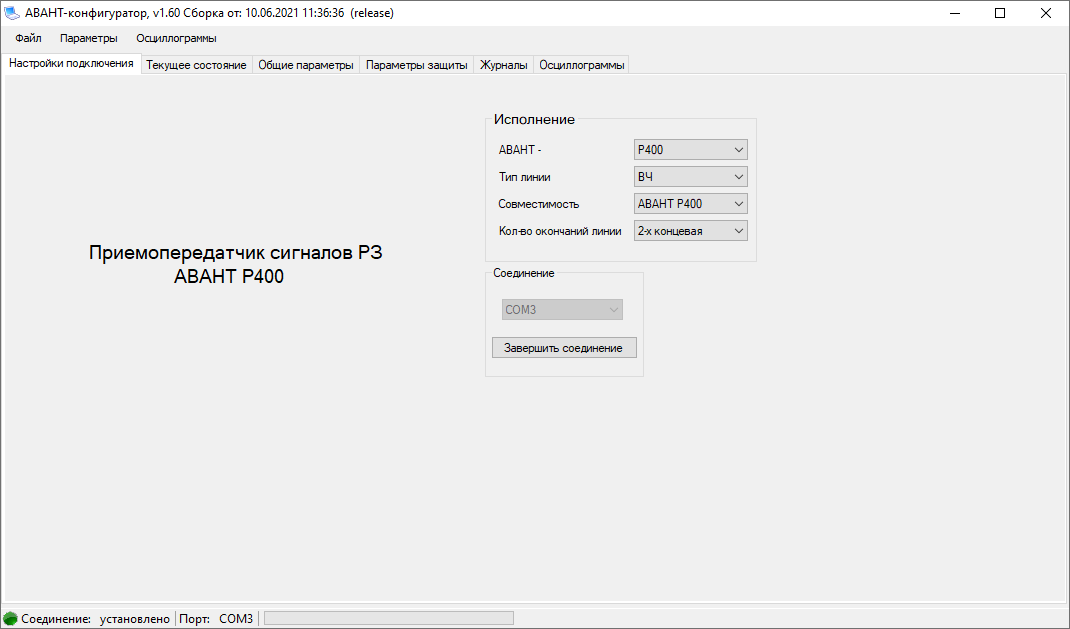
\includegraphics[width=0.8\linewidth]{configurator_connect.png}}
	
	\caption{Страница <<Настройки подключения>>}
	\label{fig:configurator_connect}
\end{figure}

Разорвать и вновь установить связь с приемопередатчиком возможно вручную с помощью кнопки <<Установить соединение>> на панели <<Соединение>> (рисунок \ref{fig:configurator_connect}), предварительно выбрав COM-порт, к которому подключен приемопередатчик. 

Вариант исполнения приемопередатчика представлен на панели <<Исполнение>>. 	
	
	
%%% ----------
\subsection{Страница <<Текущее состояние>>}	\label{ssec:configurator_state}

На данной странице (рисунок \ref{fig:configurator_state}) в режиме реального времени отображаются режим работы, текущее состояние, информация о наличии неисправностей приемопередатчика. Также на странице представлена информация об измеряемых параметрах.

\begin{figure}[H]
	\center{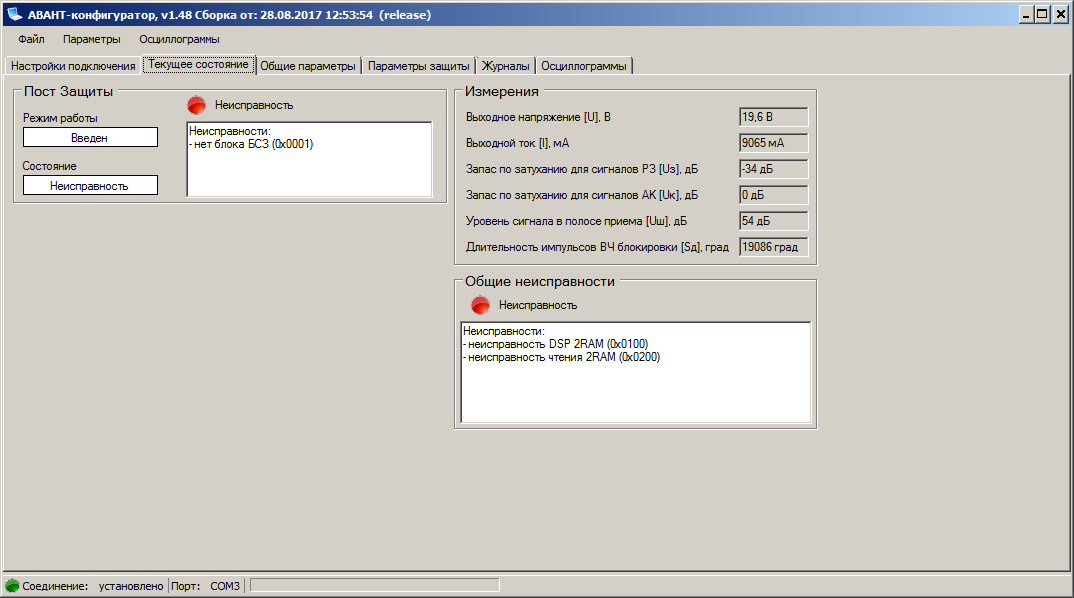
\includegraphics[width=0.8\linewidth]{configurator_state.png}}
	
	\caption{Страница <<Текущее состояние>>}
	\label{fig:configurator_state}
\end{figure}


%%% ----------
\subsection{Страница <<Общие параметры>>}	\label{ssec:configurator_param_glb}

На данной странице (рисунок \ref{fig:configurator_param_glb}) в режиме реального времени отображается режим работы приемопередатчика. На странице возможно изменение режима, изменение текущей даты и времени приемопередатчика, чтение, изменение и запись общих параметров работы приемопередатчика.

Запись параметров осуществляется только в режиме <<Выведен>>. 

\begin{figure}[H]
	\center{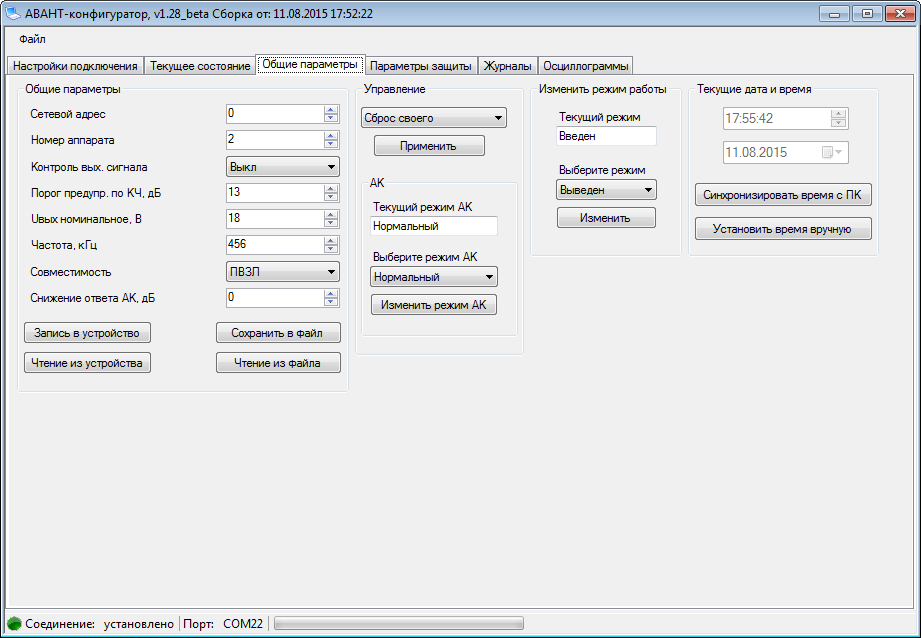
\includegraphics[width=0.8\linewidth]{configurator_param_glb.png}}
	
	\caption{Страница <<Общие параметры>>}
	\label{fig:configurator_param_glb}
\end{figure}

\textbf{Изменение режима}

Для изменения режима работы приемопередатчика необходимо на панели <<Изменить режим работы>> выбрать один из предложенных режимов и нажать на кнопку <<Изменить>>, после чего необходимо ввести пароль.
\newline

\textbf{Просмотр и изменение общих параметров}

Для того чтобы просмотреть установленные в настоящее время общие параметры работы приемопередатчика необходимо в верхней строке меню выбрать пункт <<Параметры>> $\rightarrow$ <<Чтение из устройства>> $\rightarrow$ <<Общие параметры>>. Считанные из приемопередатчика параметры отобразятся в соответствующих полях панели <<Общие параметры>>.

Для того чтобы изменить параметры необходимо ввести желаемые значения параметров и в верхней строке меню выбрать пункт <<Параметры>> $\rightarrow$ <<Запись в устройство>> $\rightarrow$ <<Общие параметры>>.
\newline

\textbf{В версиях приложения 1.53} и выше чтение и запись параметров осуществляется не раздельно по каждой группе (общие, защита), а всех сразу: в верхней строке меню пункт <<Параметры>> $\rightarrow$ <<Чтение всех параметров из устройства>> либо <<Параметры>> $\rightarrow$ <<Запись всех параметров в устройство>>.
\newline

\textbf{Сохранение и чтение общих параметров из файла}

Существует возможность сохранить измененные параметры работы приемопередатчика в файл, для этого необходимо в верхней строке меню выбрать пункт <<Параметры>> $\rightarrow$ <<Сохранить в файл>>, в появившемся окне выбрать место для сохранения, ввести имя файла и нажать <<Сохранить>>. В созданный файл будут сохранены все параметры работы приемопередатчика: общие параметры и параметры защиты.

Для того чтобы считать ранее сохраненные параметры из файла необходимо в верхней строке меню выбрать пункт <<Параметры>> $\rightarrow$ <<Загрузить из файла>>, в появившемся окне выбрать файл с параметрами и нажать <<Открыть>>. Из выбранного файла будут считаны все параметры работы приемопередатчика: общие параметры и параметры защиты. Для записи в приемопередатчик считанных из файла параметров необходимо в верхней строке меню выбрать пункт <<Параметры>> $\rightarrow$ <<Запись в устройство>> $\rightarrow$ <<Общие параметры>>. \textbf{В версиях приложения 1.53} и выше: <<Параметры>> $\rightarrow$ <<Запись всех параметров в устройство>>.
\newline

\textbf{Панель <<Управление>>}

С помощью панели <<Управление>> можно осуществить наладочный пуск передатчика сигналов защит на пять минут, запустить удаленный передатчик защиты на одну минуту, сбросить неисправности своего и удаленного приемопередатчика, включить вызывной сигнал на удаленном приемопередатчике (приглашение к переговорам), осуществить внеочередной запуск автоконтроля на своем и удаленном приемопередатчике, сбросить неисправности автоконтроля на своем и удаленном приемопередатчиках.
\newline

\textbf{Изменение значения даты и времени часов приемопередатчика}

Для изменения значения даты и времени часов приемопередатчика можно воспользоваться кнопкой <<Синхронизировать время с ПК>>, при этом дата и время в приемопередатчике установятся равными дате и времени подключенного ПК. Существует возможность установки часов вручную, для этого необходимо нажать на кнопку <<Установить время вручную>>, поля текущего времени и даты станут доступными для изменения, название кнопки изменится на <<Записать время в устройство>>. После чего необходимо ввести желаемые дату и время, нажать на кнопку <<Записать время в устройство>>. Название кнопки вновь изменится на <<Установить время вручную>>. 


%%% ----------
\subsection{Страница <<Параметры защиты>>}	\label{ssec:configurator_param_def}

На данной странице (рисунок \ref{fig:configurator_param_def}) возможны чтение, изменение и запись в приемопередатчик параметров защиты.

Запись параметров осуществляется только в режиме <<Выведен>>.

\begin{figure}[H]
	\center{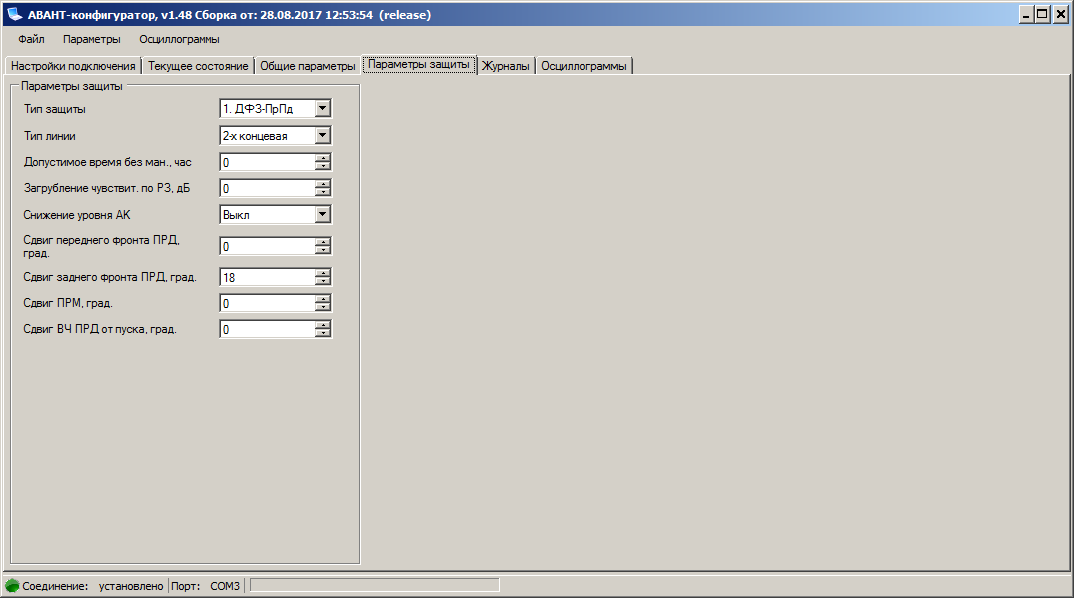
\includegraphics[width=0.8\linewidth]{configurator_param_def.png}}
	
	\caption{Страница <<Параметры защиты>>}
	\label{fig:configurator_param_def}
\end{figure}

\textbf{Просмотр и изменение параметров защиты}

Для того чтобы просмотреть установленные в настоящее время параметры работы приемопередатчика ВЧ защит необходимо в верхней строке меню выбрать пункт
<<Параметры>> $\rightarrow$ <<Чтение из устройства>> $\rightarrow$ <<Параметры защиты>>. Считанные из приемопередатчика параметры отобразятся в соответствующих полях панели <<Параметры защиты>>.

Для того чтобы изменить параметры необходимо ввести желаемые значения параметров и в верхней строке меню выбрать пункт <<Параметры>> $\rightarrow$ <<Запись в устройство>> $\rightarrow$ «Параметры защиты».

\textbf{В версиях приложения 1.53} и выше чтение и запись параметров осуществляется не раздельно по каждой группе (общие, защита), а всех сразу: в верхней строке меню пункт <<Параметры>> $\rightarrow$ <<Чтение всех параметров из устройства>> либо <<Параметры>> $\rightarrow$ <<Запись всех параметров в устройство>>. 
\newline 

\textbf{Сохранение и чтение параметров из файла}

Существует возможность сохранить измененные параметры работы приемопередатчика в файл, для этого необходимо в верхней строке меню выбрать пункт <<Параметры>> $\rightarrow$ <<Сохранить в файл>>, в появившемся окне выбрать место для сохранения, ввести имя файла и нажать <<Сохранить>>. В созданный файл будут сохранены все параметры работы приемопередатчика: общие параметры и параметры защиты.

Для того чтобы считать ранее сохраненные параметры из файла необходимо в верхней строке меню выбрать пункт <<Параметры>> $\rightarrow$ <<Загрузить из файла>>, в появившемся окне выбрать файл с параметрами и нажать <<Открыть>>. Из выбранного файла будут считаны все параметры работы приемопередатчика: общие параметры и параметры защиты. 

Для записи в приемопередатчик считанных из файла параметров необходимо в верхней строке меню выбрать пункт <<Параметры>> $\rightarrow$ <<Запись в устройство>> $\rightarrow$ <<Параметры защиты>>. \textbf{В версиях приложения 1.53} и выше: <<Параметры>> $\rightarrow$ <<Запись всех параметров в устройство>>.


%%% ----------
\subsection{Страница <<Журналы>>}	\label{ssec:configurator_journal}

В верхнем левом углу страницы <<Журналы>> (рисунок \ref{fig:configurator_journal_evt}) расположены закладки, соответствующие различным журналам:
\begin{enumerate}
	\item[1.] журнал событий – журнал общих событий и неисправностей приемопередатчика;
	\item[2.] журнал защиты – журнал работы приемопередатчика с терминалом защиты: запись управляющих воздействий от терминала (пуск передатчика, останов, манипуляция), запись фактов приема и передачи ВЧ сигналов.
\end{enumerate}

На каждой из страниц журналов расположены:
\begin{enumerate}
	\item[1.] кнопки управления: <<Чтение журнала>>, <<Сохранить в файл>>, <<Загрузить из файла>>;
	\item[2.] строка состояния, в которой отображается название журнала и количество записей в нем;
	\item[3.] таблица с записями журнала.
\end{enumerate}

\begin{figure}[H]
	\center{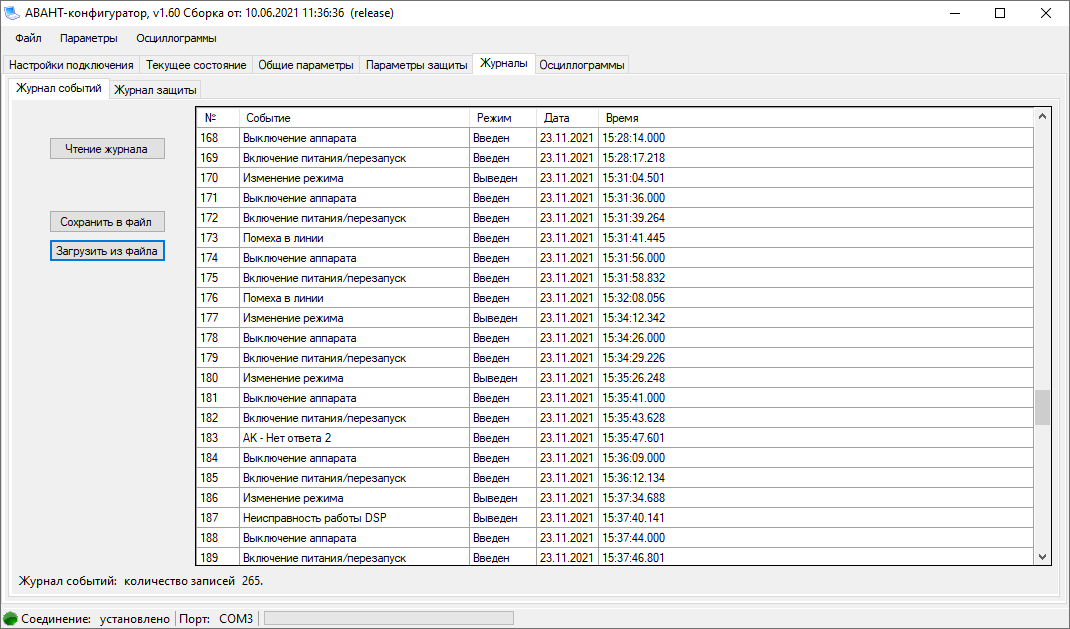
\includegraphics[width=0.9\linewidth]{configurator_journal_evt.png}}
	
	\caption{Страница <<Журналы: События>>}
	\label{fig:configurator_journal_evt}
\end{figure}

\textbf{Чтение журнала}

Для того чтобы считать журнал из приемопередатчика, необходимо нажать на кнопку <<Чтение журнала>>, при этом начнется чтение соответствующего журнала, внизу страницы в строке состояния отобразится количество записей данного журнала. После завершения чтения журнала все записи отобразятся в таблице.

Таблица журнала событий состоит из следующих колонок:
\begin{enumerate}
	\item[1.] № – номер записи;
	\item[2.] Событие – произошедшее событие, неисправность;
	\item[3.] Режим – режим работы приемопередатчика, при котором произошло событие;
	\item[4.] Дата события;
	\item[5.] Время события.
\end{enumerate}

Таблица журнала защиты состоит из следующих колонок:
\begin{enumerate}
	\item[1.] № – номер записи;
	\item[2.] Дата события;
	\item[3.] Время события.
	\item[4.] Состояние – состояние приемопередатчика, при котором произошло событие;
	\item[5.] Пуск – состояние входа <<Пуск>> на блоке КСЗ (<<0>> – в данный момент управляющего воздействия на вход нет; <<1>> – подано управляющее воздействие на вход).
	\item[6.] Останов – состояние входа <<Останов>> на блоке КСЗ (<<0>> – в данный момент управляющего воздействия на вход нет; <<1>> – подано управляющее воздействие на вход).
	\item[7.] МАН – состояние входа манипуляции на блоке КСЗ (<<0>> – в данный момент управляющего воздействия на вход нет; <<1>> – подано управляющее воздействие на вход).
	\item[8.] ПРД – состояние передатчика сигналов защит (<<0>> – передатчик остановлен, <<1>> –передатчик запущен).
	\item[9.] ПРМ – состояние приемника сигналов защит (<<0>> – приемник не принимает сигнал защиты, <<1>> – приемник принимает сигнал защиты).
	\item[10.] Выход приемника – состояние выхода приемника (<<0>> – в данный момент выход приемника не блокирован, <<1>> – выход приемника блокирован приемом сигнала защиты).
\end{enumerate}
	
В последней строке журнала выводятся дата и время считывания журнала из устройства. Дата и время считывания журнала берутся из устройства, а не из подключенного ПК.	
\newline		

\textbf{Сохранение и чтение журнала из файла}

Существует возможность сохранить каждый журнал в файл, для этого необходимо нажать на кнопку <<Сохранить в файл>>, в появившемся окне выбрать место для сохранения, ввести имя файла и нажать <<Сохранить>>. В созданный файл будет сохранен соответствующий журнал данных. 

Для того чтобы считать ранее сохраненный журнал из файла, необходимо нажать на кнопку <<Загрузить из файла>>, в появившемся окне выбрать файл с журналом и нажать <<Открыть>>. Из выбранного файла в таблицу конфигуратора будет загружен соответствующий журнал данных.


%%% ----------
\subsection{Страница <<Осциллограммы>>}	\label{ssec:configurator_oscillogram}

На данной странице (рисунок \ref{fig:configurator_oscillogram}) отображаются осциллограммы управляющих сигналов от панели защит – Пуск, Останов, Манипуляция; факты передачи и приема сигналов РЗ – ПРД, ПРМ; состояние выходной цепи приемника – Выход ПРМ.

Осциллограммы отображаются автоматически после чтения журнала защиты из приемопередатчика либо из ранее сохраненного файла с журналом защиты.

Управление осциллограммами производится с помощью мыши. Для того чтобы перемещать осциллограммы относительно меток времени, нужно нажать на правую кнопку
мыши и, удерживая ее, перемещать курсор вправо или влево.

Для того чтобы изменить масштаб осциллограммы по горизонтали, нужно нажать на левую кнопку мыши и, удерживая ее, переместить курсор вправо или влево. При этом
пунктирными линиями будет выделен отрезок времени, масштаб которого будет изменен. После чего отпустить левую кнопку мыши, выделенный отрезок времени будет растянут на все окно осциллограмм.

\begin{figure}[H]
	\center{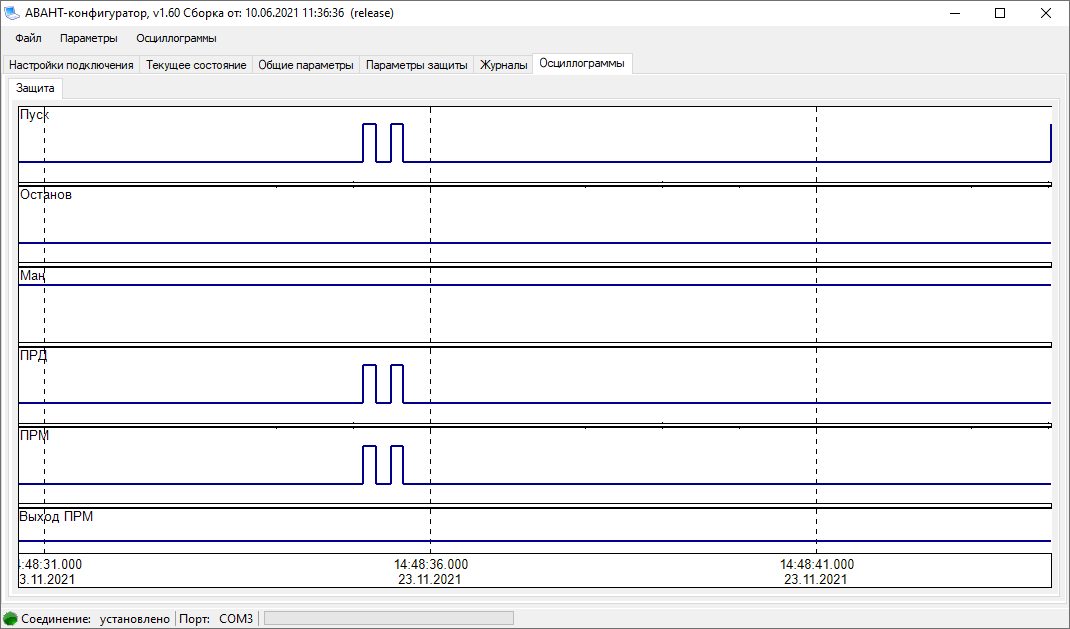
\includegraphics[width=0.9\linewidth]{configurator_oscillogram.png}}
	
	\caption{Страница <<Журналы: События>>}
	\label{fig:configurator_oscillogram}
\end{figure}

Изменять масштаб осциллограмм также возможно с помощью колеса мыши.

Для того чтобы вернуть масштаб осциллограммы в его начальное значение, необходимо в верхней строке меню выбрать пункт <<Осциллограммы>> $\rightarrow$ <<Установить масштаб по умолчанию>>.

Существует возможность сохранить осциллограммы в виде графического рисунка (файл с расширением «.jpg»), для этого необходимо в верхней строке меню выбрать пункт <<Осциллограммы>> $\rightarrow$ <<Сохранить как изображение>>, в появившемся окне выбрать место для сохранения, ввести имя файла и нажать кнопку <<Сохранить>>.
